% Chapter 2

\chapter{Sentiment Analysis} % Main chapter title

\label{Chapter2} % For referencing the chapter elsewhere, use \ref{Chapter2} 

\lhead{Chapter 2. \emph{Sentiment Analysis}} % This is for the header on each page - perhaps a shortened title

\section{Sentiment: A psychological viewpoint}

\par
Though emotion is a term used often, it has a very complex psychological background. Emotion can be described as a component process. 
There are five organismic subsystems in an individual \textit{viz. Information Processing, Support, Executive, Action, and Monitor} 
\citep*{scherer2010blueprint}. Like any system, these subsystems also have states and they keep on transiting between different states
according to the environment. Individuals respond to stimuli in the environment. Whenever an individual encounters a stimuli,
state of these subsystems change and these changes are both interrelated and synchronized. This episode is called an emotion \citep*{scherer2005emotions}.

\par
\textit{Affect} is the feeling or emotion experienced during or after the process of responding to a stimuli. This state of experience is 
called as \textit{Affective State}. Thus, emotion is one of the affective states. \textit{Mood} also can be considered as one of the affective states.
\textit{Attitude}, is one of the most important affective states. \textit{Attitude} can be defined as \textit{`` enduring, affectively colored beliefs, dispositions
towards objects or persons''}\citep*{scherer2005emotions}. \textit{Sentiment Analysis} is the nothing but the detection of attitude towards
an entity. Intuitively, we can see that it is possible to infer even the emotion. We can determine whether the user is sad, happy,
angry,\textit{etc,} if we know the attitude of the user.

%----------------------------------------------------------------------------------------

\section{Formal Problem Definition for Sentiment Analysis}

Before devising any solution to a problem, it is advisable to have concise definition of the problem first.

\subsection{Example}

Let us consider an example to define the problem,
 
\textit{"1)I went to watch the new James Bond flick, \textbf{Skyfall} at \textit{IMAX} which is the best theater in Mumbai with my brother
a month ago. 2)I really liked the seating arrangement over there. 3)The screenplay was superb and kept me guessing till the end. 
4) My brother doesn't like the hospitality in the theater even now. 5) The movie is really good and the best bond flick ever"}

\par
This is a snippet of the review for a movie named \textbf{Skyfall}. There are many entities and opinions expressed in it. 
1) is an objective statement. 2) is subjective but is intended for the theater and not the movie. 3) is a positive statement about
the screenplay which is an important aspect of the movie. 4) is a subjective statement but is made by the author's brother and also
it is about the hospitality in the theater and not the movie or any of its aspects. 5) reflects a positive view of the movie
for the author.

\par
We can see from this example that not only the opinion but the opinion holder and the entity about which the opinion has been expressed
are also very important for overall SA. Also, as can be seen from 1),4) and 5) there is also a notion of time associated with every
sentiment expressed.

\subsection{Problem Definition}

\textit{"A direct opinion (opinion about the object) is a quintuple \textbf{({o_{j}}, {f_{jk}}, {oo_{ijkl}}, {h_{i}}, {t_{l}})}, 
where \textbf{o_{j}} is an object, \textbf{f_{jk}} is a feature of the object \textbf{o_j}, \textbf{oo_{ijkl}} is the orientation 
or polarity of the opinion on feature \textbf{f_{jk}} of object \textbf{o_{j}}, \textbf{h_{i}} is the opinion holder and 
\textbf{t_{l}} is the time when the opinion is expressed by \textbf{h_{i}} "}\citep*{liu2010sentiment}.

\par
Thus we can see that the definition of sentiment analysis takes into account not only the object, opinion, and opinion holder but 
also the time and the specific feature about the sentiment is being expressed. This definition plays a very important role
in devising any approach to solve any problem related to sentiment analysis. 

\section{Types of Sentiment Analysis}

\par 
Sentiment analysis is primarily a classification task. But, we can also classify the task of sentiment analysis depending
upon various features. These features or dimensions are shown in figure \ref{fig:dimensions},

\begin{figure}[ht]
\caption{Dimensions of a Sentiment Analysis problem}
\label{fig:dimensions}
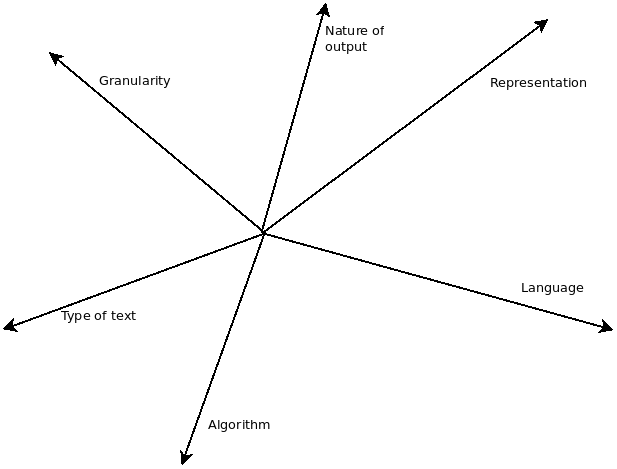
\includegraphics[width=\textwidth]{SentimentAnalysisProblemClassification.png}
\end{figure}

\clearpage

\begin{enumerate}
 \item Granularity of Text
 \item Type of text
 \item Algorithm
 \item Language
 \item Representation
 \item Nature of Output
\end{enumerate}

All these features collectively characterize a particular problem in SA. A change in even one of the features will change the
problem.

\section{Challenges}
\textit{SA} is a complex problem and has many challenges involved. In this section, an attempt is made to discuss some of the most notorious
difficulties in \textit{SA}. 

\subsection{Unstructured Text}
Text in micro-blogs, tweets, comments, and messages is unstructured. Most of the research in \textit{NLP} and many \textit{NLP} tools focus on structured
data. To adapt and use these tools for \textit{SA} is a big challenge. 

\subsection{Sarcasm}
Nowadays, many tweets and comments are sarcastic. Let us see an example on tweet, \textit{"Great! I ate too many chocolates and
gained lot of weight :)"}. This sentence will be marked as positive by almost any classifier. But, we can clearly see that this is
not a positive statement. Correctly, classifying such sentences will require context knowledge.

\subsection{Thwarting}
In a thwarted expression, the sentences which contradict the overall polarity of the document are in majority. An example is,
\textit{"The guy is a chronic drinker, he smokes weed, has drugs but is a good guy"}. The aim of thwarted expressions is to 
mislead the classifier. Detecting thwarted expressions is a very important difficulty.

\section{Applications of Sentiment Analysis}

We list some of the most important applications of \textit{SA}.

\begin{enumerate}
 \item	Classification of Tweets
 \item	Classification of Movie Reviews
 \item	Classification of Product Reviews
 \item	Analyzing market trends
 \item  Sentiment Aware Information Retrieval
 \item 	Removing subjective sentences to improve IR performance
\end{enumerate}

%----------------------------------------------------------------------------------------

\par
As we have discussed earlier, \textit{SA} is mainly a classification task. It can be thought of as a subset of a another important classification
task called \textit{Text classification}. Various approaches have been used to solve this problem. Most of them are machine learning 
based. This chapter takes a look at basic machine learning and some models in brief. Later on, combination of these models with other
techniques which take into consideration the various aspects of the \textit{text} are considered.

\section*{Approaches to Sentiment Analysis}

\section{Machine Learning}

\par

This section aims not to explain all the intricacies associated with machine learning but to provide a brief outline
which suffices for understanding future concepts. Machine learning by definition is learning from data. We have a mathematical
model, parameters of which have to be estimated from the data. By doing this we fit the model to the data provided. 
These parameters which have been \textit{learned} from the data can be said to completely define the model. Now this 
\textit{learned} model can be used for prediction or classification. In the case of \textit{SA}, \textit{Machine Learning} is used for classification
of \textit{text} as either positive, negative or neutral.

\par
The data available to us can be both labeled and unlabeled. By labeling we mean that the for an instance of the input we know
its class. Data labeling can also be called annotation. Labeled data is called annotated data. Depending upon the extent to which
the training data is labeled, we can classify the \textit{ML} techniques as follows.

\subsection{Supervised}
In this case, all the training data is a labeled. Majority of ML based techniques have this requirement that the data should be
completely labeled. The accuracy of the system decreases if the data is very small in size. This is called data sparsity problem.
They tend to over-fit if the data size is small.
\subsection{Unsupervised}
Here, the data is completely unlabeled. As opposed to supervised techniques, they do not suffer from data sparsity problem as 
the input in unlabeled.
\subsection{Semi-supervised}\label{subsection:semisupervised}
In this we have a mixture of both labeled and unlabeled data. Using the labeled data we try to annotate the unlabeled data. 
This technique is very useful if we have very sparse data.

\section{Feature Vector}
\par
Feature vector can be thought of as a way to represent the input. Some important aspects of the input are considered and used 
to represent it in the form of a vector of values. These values contain some important information which aids the classification
algorithm. 

\section{Models used for classification}
\par 
When we say we learn from the data, we actually train the model to do so. There are broadly two ways to do this. One is in a 
generative way and the other is discriminative. What do we actually mean by this? We want to infer the class of a \textit{text}.

\par
Let \textit{x} represent the input \textit{text}. We want to determine the class \textit{y} given the input \textit{i.e}, we are interested
in modeling \(p(y\mid x)\). There are three ways to do this.

\subsection{Generative Models}

\par 
One way is to model p(x, y) directly. Once we do that, we can obtain \(p(y \mid x)\) by simply conditioning on x. And we can then use decision 
theory to determine class membership \textit{i.e}, we can use loss matrix, \textit{etc}. to determine which class the point belongs to (such an assignment 
would minimize the expected loss). We can learn p(y), the prior class probabilities from the data. We can also learn \(p(x\mid y)\) from
the data using say maximum likelihood estimation (or we can Bayes estimator, if you will). Once you have p(y) and \(p(x\mid y)\), p(x, y) is 
not difficult to find out.

Bayes' rule is given as follows,

\begin{equation}
  p(y\mid x) = \frac{p(x\mid y)p(y)}{p(x)}
\end{equation}

\subsection{Discriminative Models}
Instead of modeling p(x, y), we can directly model \(p(y\mid x)\), for \textit{e.g}, in logistic regression \(p(y\mid x)\) is assumed to be of the form, 

\begin{equation}
  p(y\mid x) = \frac{1}{1 + \mathrm{e}^{(-\Sigma(wi.xi))}}
\end{equation}

All we have to do in such a case is to learn weights that would minimize the squared loss.

\par
There is a very easy technique to tell whether a model is generative or discriminative. If we can a generate new training data
using the model then it is certainly generative. In the case of generative models, the distribution \(p(x\mid y)\) is a model 
which fits the training data so it can be used to generate new data. In the case of discriminative models, this is not the case.

\subsection{Encoding a function}
We find a function f(.) that directly maps x to a class. The best example of this is decision trees. 

\section{Models}

\subsection{Naive Bayes classifier}
\par
Naive Bayes classifier is a generative classifier with strong independence assumptions. This means that all the features in feature
vector are independent of each other given the class. Despite of this very naive assumption, it gives surprisingly good results.
The parameters are estimated using the method of maximum likelihood.

Suppose we want to determine value of the class variable \textit{C} of the given input consisting of feature variables \textit{F_1,\dots,F_n}, 
it can be expressed as a conditioned probability \(p(C\mid F_1,\dots,F_n)\) using the Bayes' theorem,

\begin{equation}  
p(C\mid F_1,\dots,F_n) = \frac{p(C)p(F_1,\dots,F_n\mid C)}{p(F_1,\dots,F_n)}
\end{equation}

To use this equation for classification of a given input \textit{x} which is represented by a feature vector \textit{(F_1=f_1,\dots,F_n=f_n)},
the following equation is used,

\begin{equation}
class(f_1,\dots,f_n) = \arg\max_c p(C=c) \prod_{i=1}^{n} p(F_i = f_i \mid C=c) 
\end{equation}

\par
The main advantage of Naive Bayes is that it gives remarkably high accuracy for relatively small data sets because of the independence
assumption. 

\subsection{Maximum Entropy}
\par
Maximum Entropy more commonly known as \textit{MaxEnt} is a discriminative classifier. As it is a discriminative classifier, here we find out 
the conditional distribution of the class variable. The basic principle underlying maximum entropy is that without external knowledge
one should prefer distributions which are uniform and have maximum entropy. Using the training data, constraints on the distribution 
are derived which can be used to infer where the distribution should be minimally non-uniform. These constraints represent the expected
values of the features \citep*{nigam1999using}. In Text classification, \textit{MaxEnt} estimates the conditional distribution of the class label
given the \textit{text}. Representation of the \textit{text} is mostly in terms of word count features or word presence features.

 
Let \textit{f} be the features that link the observation \textit{x} to the class \textit{c}. A feature in this case is a function denoted
by \textit{f_i(x,c)} with a bounded real value. Also, let \textit{X} denote the collection of \textit{texts}. The aim of \textit{MaxEnt} is to
restrict the model distribution to have the same expected value for each such feature as is seen in the training data \textit{X}. 
This means that the learned conditional distribution \(p(c \mid x)\) must satisfy the following property, 

\begin{equation}\label{eqn:property}
 \frac{1}{|X|} \sum_{x \in X} f_i(x, c(x)) = \sum_x p(x) \sum_c p(c \mid x)f_i(x,c)
\end{equation}

equation ~\ref{eqn:property} reduces to the following form as we are not interested in modeling the collection \textit{X} here.

\begin{equation}\label{eqn:newproperty}
 \frac{1}{|X|} \sum_{x \in X} f_i(x, c(x)) = \frac{1}{|X|} \sum_{x \in X} \sum_c p(c \mid x)f_i(x,c)
\end{equation}

Feature identification is very important in this case. Using the training data, expected value of features is used as a constraint
for the model distribution. A class label for which most of these constraints are satisfied is the class of the given input \textit{x}.

\subsection{SVM}
A basic \textit{SVM} is a non-probabilistic binary linear classifier which given an input data predicts which of the two possible classes
forms the output.

\section{Usage in SA}

We have covered lot of basics to easily understand some of the techniques used for SA. We start with a basic bag of words model 
and then move on to more advanced techniques which incorporate the attributes of \textit{text}. Discourse based technique is 
discussed followed by a technique which makes use of minimum cut of a graph. These are followed by an unsupervised method which
makes use of a search engine called \textit{Alta Vista} to determine the semantic orientation of the \textit{text}. The last method
we discuss is a semi-supervised method which aims to perform ternary classification of sentences. 

\subsection{Bag of Words}

In a Bag of Words model, the feature vector is just a unigram model which is used to represent the presence or absence of a word.
Let us consider an example sentence, \textit{"I hate to play football"} and suppose the vocabulary \textit{V} is \(\left\{I, You, like, 
hate, to, for, play, dance, football, cricket\right\}\). In this case,  the feature vector will be \textit{(1,0,0,1,1,0,1,0,1,0)}.
We can see that here every word is a feature. In addition, it makes use of list of positive and negative words. If a word is positive
then the value corresponding to that feature is +1 and if it is negative the value is -1. Thus for the example is our case, the 
feature vector after making use of this dictionary becomes \textit{(1,0,0,-1,1,0,1,0,1,0)}. This feature vector is nothing but
a representation of the input. If sum of all the values is positive then the sentence has positive polarity and if it is less than
zero then it has negative polarity. For our example, it turns out that the sentence is negative. The accuracy of such a system though 
is not very good, around 65 \%.

On the other hand, If this input is fed to a default classifier like \textit{NB}, \textit{SVM} or \textit{MaxEnt} then it is shown to have a considerable increase
in accuracy\citep*{go2009twitter}. In \citep*{go2009twitter}, they conducted various experiments and got the results as shown in table
\ref{table:classifierAccuracy}

\begin{table}
 \caption{Classifier Accuracy}
 \begin{center}
 \begin{tabular}{| c | c | c | c | c | }
  \hline
  Features 		& Keywords & Naive Bayes & MaxEnt & SVM \\ \hline
  Unigram  		& 65.2 & 81.3 & 80.5 & 82.2 \\ \hline
  Bigram 		& N/A & 81.6 & 79.1 &78.8 \\ \hline
  Unigram + Bigram 	& N/A & 82.7 & 83.0 & 81.6 \\ \hline
  Unigram + POS 	& N/A & 79.9 & 79.9 & 81.9 \\
  \hline
 \end{tabular}
 \end{center}
 \label{table:classifierAccuracy}
\end{table}

\subsection{Adding Discourse information}

\par
Discourse elements have a sentiment changing impact on sentences. Let us consider an example,

\begin{center} \textit{"The screenplay was good but I didn't like the movie"}\end{center}

\par
Feature vectors discussed in the previous section won't be able to encode the information in such sentences. Using Bag of Words 
model can result in classification to a completely opposite polarity. To detect the polarity of such a sentence, detection of 
discourse elements and determining their effect is very important. Many approaches for this are present but all of them are for 
structured data and on most of the micro-blogging sites, the content is unstructured. Unstructured data is the main reason that 
many sentiment analysis tools make use of bag-of-words model. 


\par
To solve this problem, it is important to categorize the various types of discourse relations and find out the semantic operators 
which play a major role. In \citep*{mukherjeesentiment}, discourse relations have been categorized and many examples have been given to emphasize on 
some specific relation. Also, the semantic operations influencing the polarity have been explained. The algorithm then takes
into consideration all these attributes to create a feature vector. A weight is assigned to each valence shifter taking into 
consideration its position w.r.t the discourse element. Also, the polarity/sense of a particular word is flipped depending upon 
its position. It also makes an attempt to take into account the impact of  modals, which should lower the weight in some cases. 
The feature vector thus consists of weight, polarity, flipping and modality values for each word in the sentence. Words having 
zero weight have do not affect the polarity in any way and are thus ignored while calculation. The Feature vector thus created can be used for calculation the sentiment behind the sentence.
Two methods have been used, one is Lexicon based classification and the other is \textit{SVM} classification. In the \textit{SVM} classification, 
words with the same root are represented with a single vector. Also, special handling of \textit{emoticons} is present. \textit{WSD} is also used
to determine the exact sense of each word. The results show that this algorithm outperforms all the methods by a margin which has
statistically significant. Also, since this is lightweight and extends the baseline bag-of-words model, the performance of the 
system is very good. 

\subsection{Influence of Objective sentences on Classification}\label{section:subanalysis}

In \citep*{pang2004sentimental}, they have attempted to classify movie reviews as positive or negative. In this case the granularity
of the \textit{text} is a \textit{document}. Movie reviews often contain description of the plot. This description might contain
polar sentences but they have no relation whatsoever with the review about the movie. These sentences don't help in describing
about how good or bad the movie is. Consider the following example sentence from the review of a recent movie,

\textit{"The action follows Jean Valjean, a former convict, as he flees Javert, a fanatical police officer, through
a version of 19th-century France peopled with various grotesques, victims and tarnished saints."}

As we can see this sentence has a number of words with negative polarity. This will be classified as a negative sentence which 
might lead to the review as a whole being classified as negative. But, we know that this sentence is from the description of the 
plot and is not an opinion/review about the movie. To solve this problem, we need to identify which sentences are objective and discard them.
Subjective sentences in this scenario mean those sentences which are meant to describe the plot or contain some factual information.

The approach followed in \citep*{pang2004sentimental} has three steps,

\begin{enumerate}
 \item 	Label the sentences in the document subjective or objective
 \item The objective sentences are discarded. This extraction is based on minimum cut formulation which integrates inter-sentence contextual
information with Bag of Words model
 \item A standard machine learning approach is applied to the extract for polarity classification
\end{enumerate}

\subsubsection*{Subjectivity Detection}

This is the first step in their approach. They try to identify subjective sentences. For this, they have made use of cut-based
classification. Also, coherence of sentences is also taken into consideration. Coherence means that subjectivity status of two 
sentences close to each other may be same.

\textit{"I really loved the screenplay of this one. Award Winning Directors are often good at making such movies"}

As we can see from this example, two coherent sentences should ideally be classified under the same class.

\subsubsection*{Cut-based classification}

Let \(x_1,\dots,x_n\) be the sentences in the \textit{document}. Also, let \(C_1,\dots,C_k\) be the classes into which the sentences are to be classified.
There are two important sources of information which can aid the classification. 

\begin{enumerate}
 \item Individual scores: \(ind_i(x_i)\) - Preference of each \(x_i\) for being in class \(C_j\)
 \item Association scores: \(asso(x_i , x_j)\) - Estimate of how important it is that \(x_i\) and \(x_j\) are in the same class
\end{enumerate}

So, in the cut based classification penalizes if tightly associated items are put in different classes. So, taking into consideration,
the objective is to minimize the cost given below.

\begin{equation}
 \sum_{x\in C_1} ind_2(x) + \sum_{x\in C_2} ind_1(x) + \sum_{x_i \in C_1, x_k \in C_2} assoc(x_i,x_k)
\end{equation}

Now, we can see that this problem in intractable as there are 2^n possible partitions of x_i's. This minimization problem can be solved by
building an undirected graph \(G\) with vertexes \({ v_1, v_2 , v_3 ,\dots, v_n , s, t }\) . The last two are source and the sink and represent the two classes

The graph consists of following edges

\begin{enumerate}
  \item \(n\) edges \((s, v_i )\) with weight \(ind_1 (x_i )\)
  \item \(n\) edges \((t, v_i )\) with weight \(ind_2(x_i)\)
%   \item \( n \choose 2 \) edges \((v_i , v_k )\) each with weight \(assoc(x_i , x_k )\)
\end{enumerate}

A cut \((S, T)\) of \(G\) is a partition of its nodes into sets \(S = {s} \cup S\) and \(T = {t} \cup T\) where \(S\) does not contain 
\(s\) and \(T\) does not contain \(s\). Its cost \(cost(S, T )\) is the sum of the weights of all edges crossing from \(S\) to \(T\). 
A minimum cut of \(G\) is one of minimum cost.

\subsubsection*{Polarity classification}

Using the cut-based classification, we get the subjective sentences in the movie review. This extract is the fed to default polarity classifiers
which in this case are \textit{NB} and \textit{SVM}. The feature vector used for them is unigram based. 

\subsubsection*{Significance}

A cleaner document can be obtained by extracting only the subjective information. The accuracy of the polarity classification
improves as they don't get irrelevant data.The performance of the system will improve as it has less text to work on.

\subsection{Unsupervised semantic orientation}

A completely unsupervised approach to SA has been used in \citep*{turney2002thumbs}. It is aimed for classification of reviews about
products, automobiles, review, \textit{etc}. The approach used has three steps.

\begin{enumerate}
 \item Find phrases in the review containing adjectives and adverbs
 \item Find semantic orientation of such phrases
 \item Take avg of semantic orientation. If it is positive then \textit{Thumbs up} else \textit{Thumbs down}
\end{enumerate}

\subsubsection*{Step 1}

Extract phrases containing adjectives or adverbs. Adjectives are good indicators of subjectivity. Adjectives in isolation have 
insufficient context to determine semantic orientation. \textit{e.g}, \textit{“unpredictable”} when applied to \textit{“steering”} in a car 
review has negative semantic orientation. On the other hand \textit{“unpredictable plot”} in a movie review has positive orientation.

Therefore the algorithm uses 2 consecutive words where one is adjective/adverb and the other provides context.

\subsubsection*{Step 2}

\subsubsection*{Point-wise Mutual Information (PMI)}
Point-wise Mutual Information between two words word1 and word2 is defined as

\begin{equation}
PMI(word_1,word_2) = log_2 \Bigg[ \frac{p(word_1 \wedge word_2)}{p(word_1)p(word_2} \Bigg]
\end{equation}

where \(p(word_1 \wedge word_2 )\) is the probability that \(word_1\) and \(word_2\) co-occur.

\subsubsection*{Semantic Orientation}

Semantic orientation of a phrase is given by,

\begin{equation}
\label{eqn:SO}
SO(phrase) = PMI(phrase, excellent) - PMI(phrase,poor)
\end{equation}
  
The \textit{PMI} are estimated by issuing queries to a search engine which explains the \textit{IR} in \textit{PMI-IR}. It notes 
the number of hits to calculate the probability values. The search engine used in this case was \textit{AltaVista}.

After some algebraic simplifications and using the fact that \(p(phrase,excellent) = \textit{hits(phrase NEAR excellent)} \), 
equation \ref{eqn:SO} reduces to the following form:

\begin{equation}
SO(phrase) = log_2 \Bigg[ \frac{\textit{hits(phrase NEAR excellent)hits(poor)}}{\textit{hits(phrase NEAR poor)hits(excellent)}} \Bigg]
\end{equation}

Here, \textit{hits(query)} stands for the number of hits returned by the query.

\subsubsection*{Step 3}

In this step, average of the semantic orientations of all the phrases is taken.

\begin{itemize}
  \item If the avg is positive then Thumbs Up.
  \item If the avg is negative then Thumbs Down.
\end{itemize}

\subsubsection*{Observations}

After experiments were conducted, following observations were made.

\begin{itemize}
 \item Movie Reviews are hard to classify because a good movie might contain unpleasant scenes. Description of such scenes might decrease the
	semantic orientation.
 \item Accuracy did not increase just by accounting for this bias using a constant value. Just as positive reviews have description of unpleasant scenes, negative reviews might
	contain description of pleasant scenes.

\end{itemize}

\subsubsection*{Limitations}

This approach has some limitations as can be seen from the architecture. 

\begin{itemize}
 \item Queries search engine to calculate semantic orientation of each phrase.
 \item Every phrase is given equal importance. There should be a weighted sum.
 \item The performance in case of movie reviews is not good because it does not take into account the fact that the whole is not
	necessarily a sum of parts as pointed out in section. \ref{section:subanalysis}
\end{itemize}

\subsection{Semi-supervised}

A semi-supervised approach for detecting term orientation was used in \citep*{esuli2006determining}. 
In \citep*{esuli2006determining}, they have tried to perform a ternary classification of terms as objective, positive, or negative. 
The motivation behind this study is that in most works which determine the term orientation, it is assumed that we already know 
whether it a subjective term or not. So, we assume that a lexical resource of subjective/objective terms is available. This is not 
the case. 

Semi-supervised was discussed briefly in section \ref{subsection:semisupervised}. Semi-supervised can be depicted as shown in figure 2.1

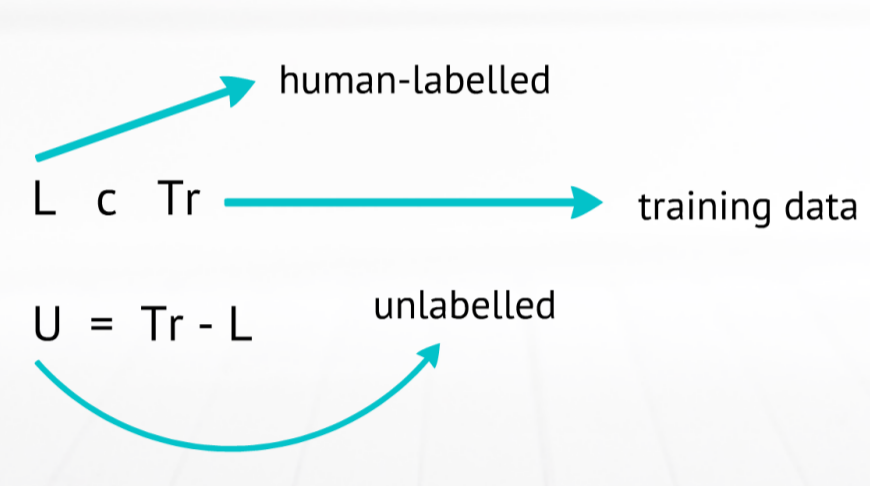
\includegraphics[width=\textwidth]{semisupervised}

\begin{center}
 Figure 2.1 Training Data in semi-supervised learning
\end{center}

 
The unlabeled data has to be labeled and it should also be used for training. The labeled usually is called as seed set.
In \citep*{esuli2006determining}, they have made used of synonymy-antonymy relations of the wordnet to create the training data. 

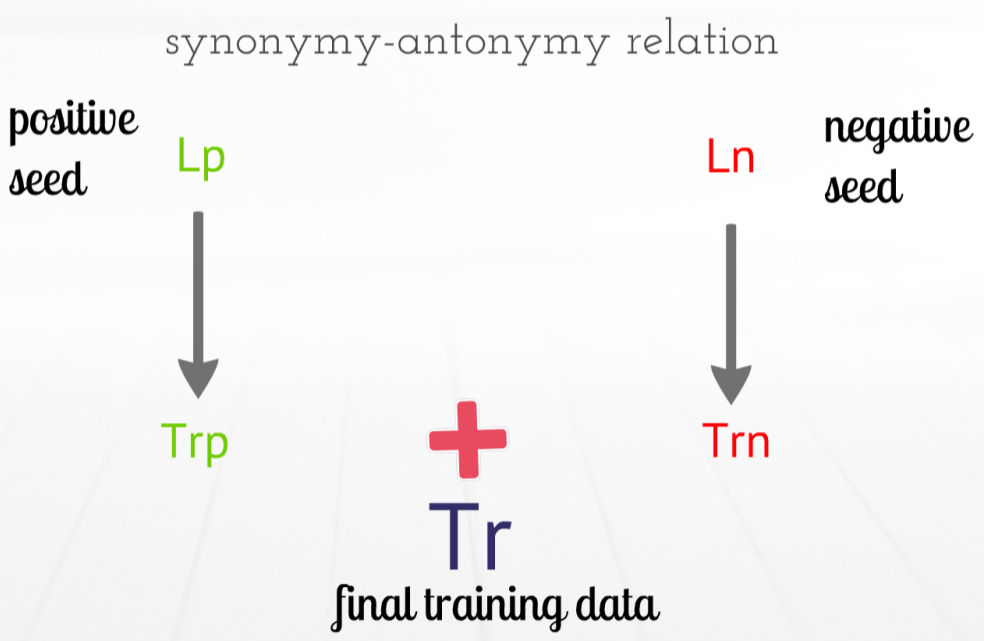
\includegraphics[width=\textwidth]{synonymyantonymyrelation}
\begin{center}
 Figure 2.2 Using synonymy-antonymy relation for labeling unlabeled data
\end{center}


As we can see, we start with very small seed sets in this case, each containing only one element. The exact procedure is shown in 
the figure 2.3.

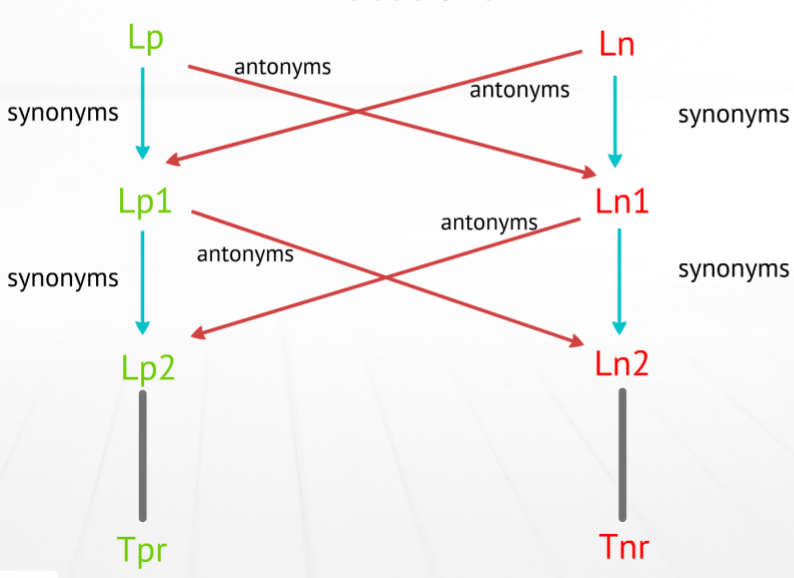
\includegraphics[width=\textwidth,height=0.6\textwidth]{procedure}
\begin{center}
 Figure 2.3 Procedure for labeling unlabeled data using synonymy-antonymy relation
\end{center}


\par
After getting all the training data, a textual representation for each term is generated by collating all the wordnet glosses
for that term. A cosine normalized \textit{TF-IDF} representation is used as the feature vector. The result obtained by the approaches used
in this paper were not that accurate and they show that algorithm used for term orientation when used for ternary classification
perform badly and need improvement.

\section*{SUMMARY}

In this chapter we introduced \textit{Sentiment Analysis}. The motivation behind this work was discussed. A psychological viewpoint of 
\textit{SA} was explained. A formal problem definition of sentiment analysis was given. This was followed by depicting the various 
dimensions of a problem in \textit{SA}. Prevalent challenges in sentiment analysis were discussed briefly and some major applications were
listed. Then we started with the basics of Machine Learning. Then we explained the various approaches and techniques used
in ML. We explained what is a feature vector. Moving forward, we tried to understand the different models used in ML. Works using
all these techniques were explained.

In the next chapter we will discuss information retrieval and the focus on corpus models, mainly \textit{LDA}.

\clearpage